\documentclass{article}
\usepackage{../../Self_Style}

%setup hyperlink within pdf
\hypersetup{
    colorlinks=true,
    linkcolor=blue,
    filecolor=magenta,      
    urlcolor=cyan,
    pdftitle={Overleaf Example},
    pdfpagemode=FullScreen,
}

\title{Phys 20AL Lab Report Week 1: Pendulum}
\author{Zih-Yu Hsieh}
\date{\today}

\begin{document}
\maketitle

\tableofcontents

\hfil

\section{Introduction and Goal of the Experiment}
%explain what pendulums are, basic formulas, and the aim for the experiment (study relationships between length, mass, period of the pendulum)+ derive 
Under humans' observations, Pendulum is a physical system that obtains similar time period for each cycle when the amplitude of the cycles considered are small enough relative to the arm of the pendulum. Equivalently, one can also say this similarity occurs when the angle of the arm away from the bottom (the equilibrium point) is approximately $0$.

Under small angle approximation, the formula physicists derived for the pendulum's period is $\tau\approx 2\pi\sqrt{\frac{g}{l}}$ second (unit abbreviated as s), given that $l$ is the length of the arm of the pendulum (in units of meters m), and $g \approx 9.807$ m/s$^2$ (meters per second square) is the gravitational acceleration near Earth's surface.

The aim for this experiment includes:
\begin{itemize}
    \item Observe the (human observable) relationships between the mass $m$, the arm length $l$, and the period $\tau$ of a simple pendulum.
    \item Calculate how well the formula of period mentioned above approximates the actual period under fixed small angle.
    \item Use the experimental data to calculate gravitational acceleration $g$ near Earth's surface.
\end{itemize}

\pagebreak

\section{Experimental Setup (fxxk you image problem)}
The equipments for this experiment include: A stand, a protractor, a clip, a tape measure, a timer, a mass scale, a string with negligible mass, and multiple spherical weighted objects (each with different mass, depending on the lab equipment's availability).

The setup of the experiment goes as follow:
\begin{itemize}
    \item[1.] Fix the stand at the edge of the lab table, and fix the protractor horizontally on the top of the stand for measuring the pendulum arm's angle away from the equilibrium point.
    \item[2.] Tie / fix one end of the string to the clip, and clip it onto the stand. This is used for controlling the length of the pendulum's arm (or the length of the string that is hanged under the pivot).
    \item[3.] Put the other end of the string through a hole on the top of the stand, which serves as a pivot for the pendulum.
    \item[4.] Hang the spherical object(s) that serve as the mass of the pendulum at the end of the string that passes through the hole in 3.
\end{itemize}
\begin{figure}[h!]
    \centering
    \begin{subfigure}[t]{0.3\textwidth}
        \centering
        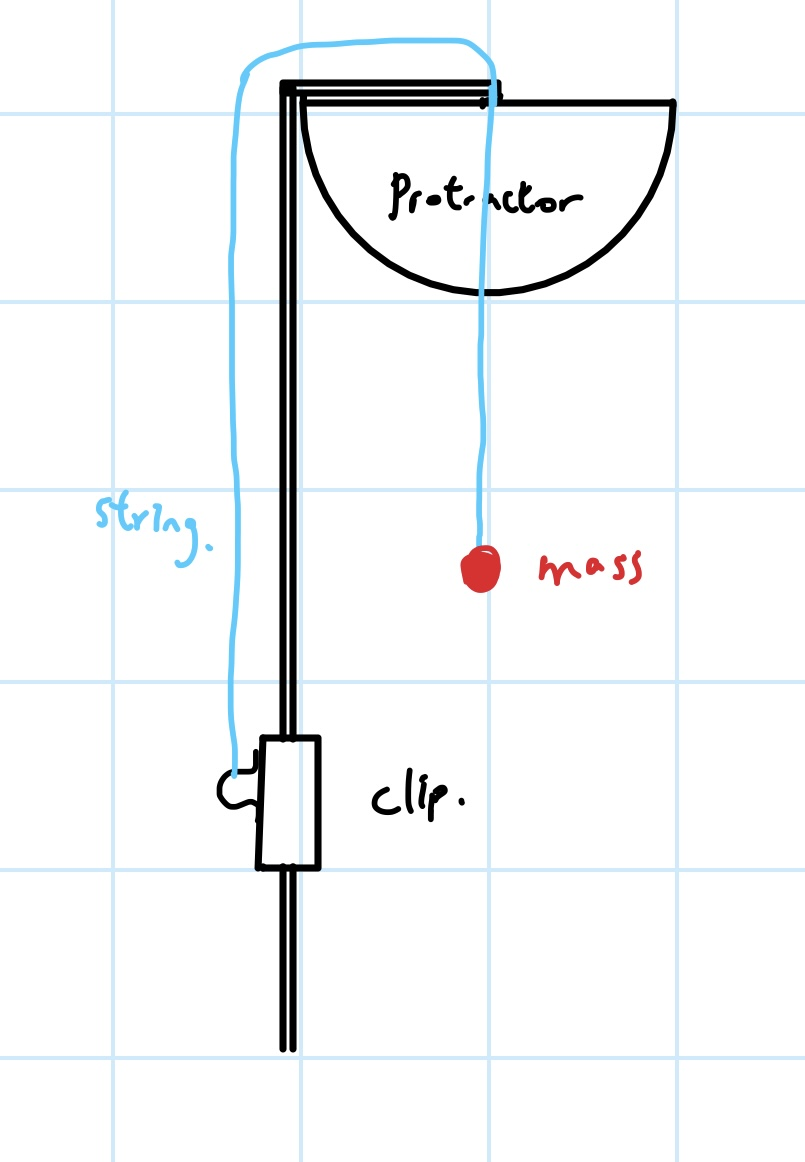
\includegraphics[width=\linewidth]{setup_sketch.png}
        \caption{Simplified Sketch of the Equipment Setup}
        \label{fig:sketch_setup}
    \end{subfigure}%
    \hfil 
    \begin{subfigure}[t]{0.3\textwidth}
        \centering
        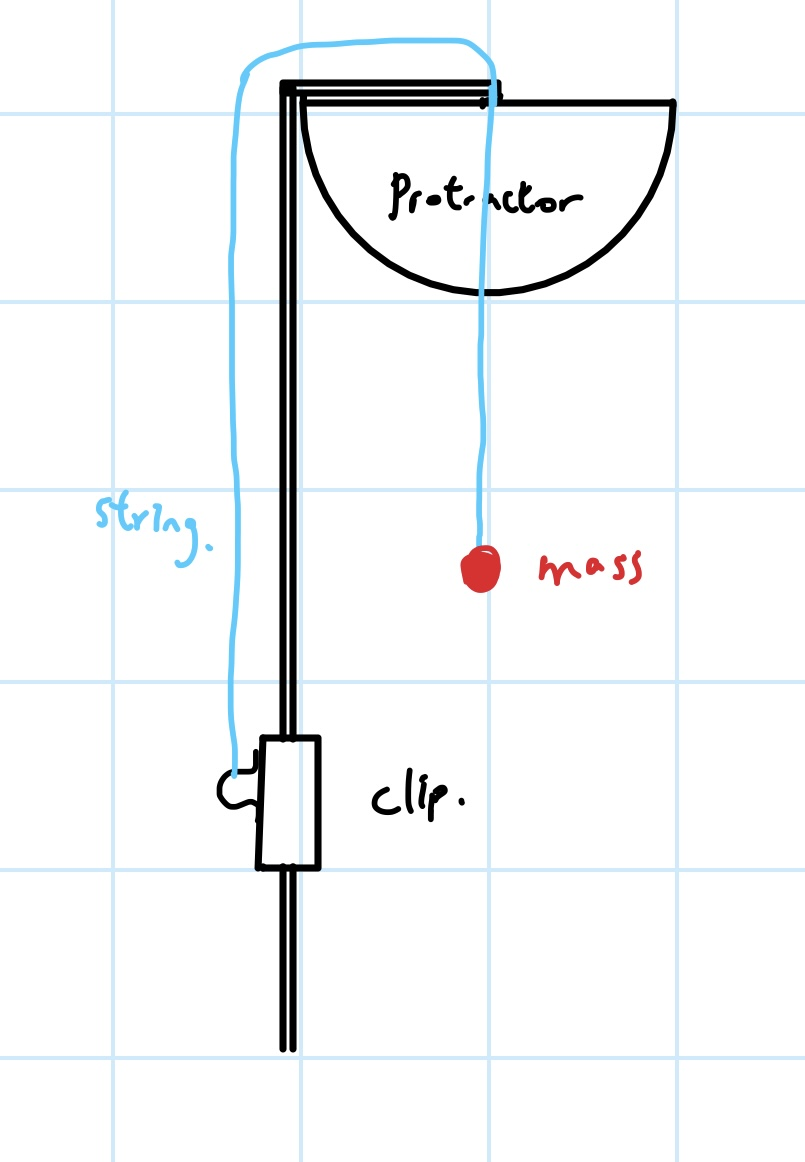
\includegraphics[width=\linewidth]{setup_sketch.png}
        \caption{Photo of the Equipment Setup}
        \label{fig:physical_setup}
    \end{subfigure}
\end{figure}

\pagebreak

\section{Procedure and Methods of Measurement}
For each individual trial we'll record the length $l$ of the pendulum using tape measure, use the mass scale to measure the hanged mass $m$ on the pendulum, and use the timer to measure the period $\tau$ of the pendulum.

The independent variables include length $l$ and mass $m$ of the pendulum, which we'll test trials for each of the following combination:
\begin{itemize}
    \item The lengths of the pendulum used are $0.3$m, $0.4$m, $0.5$m, and $0.6m$. 
    \item The masses of the pendulum used are $5.5$g, $20$g, $66$g, and $71.5$g (based on the provided objects in the lab). 
\end{itemize}
The dependent variable of the experiment is the period $\tau$ of the pendulum, while the rest of the factors are considered as controlled variables.

For the experiment, we'll follow the procedure below:
\begin{itemize}
    \item[1.] First, choose a mass for the pendulum, hang it onto the string, then fix a length for the pendulum by adjusting the position of the clip.
    \item[2.] Raise the pendulum till it is $10^\circ$ away from equilibrium (check it with the protractor) and release.
    \item[3.] Wait for the pendulum to complete $5$ cycles, then record the period for the $6^\textmd{th}$ cycle using the timer.
    \item[4.] Repeat Step 2 and 3 five times with fixed mass and length.
    \item[5.] Change the length of the pendulum to a different one await to be experimented with, and repeat Step 2 to 4 for each length.
    \item[6.] Change the mass of the pendulum to a different one await to be experimented with, and repeat Step 2 to 5 for each desired mass.
\end{itemize}
The purpose is to observe the effect of the pendulum length on the period of the pendulum under fixed mass and other conditions, then compare the variation of the overall effects when masses are changed.

\pagebreak

\section{Experimental Data and Tables}
\begin{table}[ht!]
    \centering

    % First row
    \begin{subtable}[t]{0.45\textwidth}
        \centering
        \caption{Mass: 5.5g}
        \begin{tabular}{c||c|c|c|c|c}
            \toprule
            \diagbox[width=3cm,height=1cm]{Length (m)}{Trial} & 1 & 2 & 3 & 4 & 5 \\
            \midrule
            0.3 & 1.08 & 1.04 & 1.13 & 1.15 & 1.06 \\
            \hline
            0.4 & 1.26 & 1.33 & 1.23 & 1.24 & 1.18 \\
            \hline
            0.5 & 1.41 & 1.48 & 1.38 & 1.43 & 1.39 \\
            \hline
            0.6 & 1.49 & 1.53 & 1.49 & 1.58 & 1.48 \\
            \bottomrule
        \end{tabular}
        \label{tab:mass_5.5g}
    \end{subtable}
    \hfill
    \begin{subtable}[t]{0.45\textwidth}
        \centering
        \caption{Mass: 20g}
        \begin{tabular}{c||c|c|c|c|c}
            \toprule
            \diagbox[width=3cm,height=1cm]{Length (m)}{Trial} & 1 & 2 & 3 & 4 & 5 \\
            \midrule
            0.3 & 1.09 & 1.03 & 1.09 & 1.09 & 1.13 \\
            \hline
            0.4 & 1.06 & 1.29 & 1.29 & 1.19 & 1.24 \\
            \hline
            0.5 & 1.34 & 1.43 & 1.44 & 1.46 & 1.43 \\
            \hline
            0.6 & 1.59 & 1.51 & 1.58 & 1.51 & 1.53 \\
            \bottomrule
        \end{tabular}
        \label{tab:mass_20g}
    \end{subtable}

    \vspace{1em}

    % Second row
    \begin{subtable}[t]{0.45\textwidth}
        \centering
        \caption{Mass: 66g}
        \begin{tabular}{c||c|c|c|c|c}
            \toprule
            \diagbox[width=3cm,height=1cm]{Length (m)}{Trial} & 1 & 2 & 3 & 4 & 5 \\
            \midrule
            0.3 & 1.01 & 1.08 & 1.11 & 1.04 & 1.09 \\
            \hline
            0.4 & 1.19 & 1.26 & 1.29 & 1.24 & 1.28 \\
            \hline
            0.5 & 1.34 & 1.43 & 1.44 & 1.46 & 1.43 \\
            \hline
            0.6 & 1.48 & 1.58 & 1.54 & 1.48 & 1.63 \\
            \bottomrule
        \end{tabular}
        \label{tab:mass_66g}
    \end{subtable}
    \hfill
    \begin{subtable}[t]{0.45\textwidth}
        \centering
        \caption{Mass: 71.5g}
        \begin{tabular}{c||c|c|c|c|c}
            \toprule
            \diagbox[width=3cm,height=1cm]{Length (m)}{Trial} & 1 & 2 & 3 & 4 & 5 \\
            \midrule
            0.3 & 1.11 & 1.03 & 1.06 & 1.08 & 1.07 \\
            \hline
            0.4 & 1.23 & 1.23 & 1.34 & 1.21 & 1.23 \\
            \hline
            0.5 & 1.39 & 1.39 & 1.41 & 1.33 & 1.43 \\
            \hline
            0.6 & 1.54 & 1.54 & 1.53 & 1.51 & 1.58 \\
            \bottomrule
        \end{tabular}
        \label{tab:mass_71.5g}
    \end{subtable}

    \caption{Measured oscillation periods (unit: second s) for different masses and string lengths}
    \label{tab:period_table}
\end{table}

\section{Data Analysis}

\section{Conclusion}

\end{document}